\documentclass[11pt,a4paper]{article}

\usepackage[margin=2.5cm]{geometry}
\usepackage{graphicx}
\usepackage{booktabs}
\usepackage{longtable}
\usepackage{array}
\usepackage{hyperref}
\usepackage{xcolor}
\usepackage{listings}
\usepackage{fancyhdr}
\usepackage{enumitem}
\usepackage{caption}
\usepackage{float}

\hypersetup{
  colorlinks=true,
  linkcolor=black,
  urlcolor=black,
  citecolor=black,
  filecolor=black,
  allcolors=black
}

\color{black}

\definecolor{codebg}{RGB}{248,248,248}
\lstset{
  basicstyle=\ttfamily\small,
  backgroundcolor=\color{codebg},
  breaklines=true,
  frame=single,
  rulecolor=\color{gray!40}
}

\pagestyle{fancy}
\fancyhf{}
\lhead{UCSC QA Automation}
\rhead{R.P.S.R. Ranasinghe (22020782)}
\cfoot{\thepage}

\title{\textbf{UCSC Practical Take-Home Assignment}\\QA Automation\\[0.4em]
\large OrangeHRM Open Source Demo}
\author{R.P.S.R. Ranasinghe\\Student ID: 22020782}
\date{August 2026}

\begin{document}
\maketitle
\thispagestyle{empty}

\begin{center}
\fbox{\parbox{0.92\textwidth}{
\textbf{Website:} \url{https://opensource-demo.orangehrmlive.com/web/index.php/auth/login}\\
\textbf{GitHub:} \url{https://github.com/SeniruR/QA-Automation-ASQA}\\
\textbf{Video:} \url{https://drive.google.com/file/d/1LVjVxsYdon5JppayyAF42kQZpBJ2Ra5C/view?usp=sharing}\\
\textbf{Stack:} Java 17, Selenium WebDriver 4, TestNG, Maven, Page Object Model
}}
\end{center}

\tableofcontents
\newpage

% ============================================================
\section{Selected Website}
% ============================================================

\begin{table}[H]
\centering
\begin{tabular}{@{}ll@{}}
\toprule
\textbf{Item} & \textbf{Detail} \\
\midrule
Application & OrangeHRM OS Demo (v5.x) \\
URL & \url{https://opensource-demo.orangehrmlive.com/web/index.php/auth/login} \\
Approval & Lecturer approved \\
Why this site & Public HRMS demo with Login, Dashboard, PIM, Admin, Leave modules \\
\bottomrule
\end{tabular}
\end{table}

\noindent\textbf{Demo credentials:} Username \texttt{Admin} / Password \texttt{admin123}

% ============================================================
\section{Requirement Analysis}
% ============================================================

\subsection{Application Objectives}
OrangeHRM is an open-source Human Resource Management System used to manage employees, leave, time, and system users. The demo site allows exploration of HR workflows through a web UI.

\subsection{Target Users}
\begin{itemize}[noitemsep]
  \item \textbf{System Admin} - manage users, roles, job titles, organisation structure
  \item \textbf{HR / PIM user} - add, search, and edit employee records
  \item \textbf{Employee} - view personal info and apply leave (role-dependent)
\end{itemize}

\subsection{Key Features Observed}
\begin{enumerate}[noitemsep]
  \item Authentication (login / logout)
  \item Dashboard with widgets and side navigation
  \item PIM - employee list, add employee, search filters
  \item Admin - system users, job, organisation
  \item Leave - apply, assign, list leave
  \item Additional modules: Time, Recruitment, My Info, Performance, Directory
\end{enumerate}

\subsection{Assumptions}
\begin{itemize}[noitemsep]
  \item Demo site remains publicly available during the assignment window
  \item Default Admin credentials remain \texttt{Admin} / \texttt{admin123}
  \item Microsoft Edge or Google Chrome available for automation
  \item Shared demo data may be reset or changed by other users
\end{itemize}

\subsection{Risks and Mitigation}
\begin{table}[H]
\centering
\small
\begin{tabular}{@{}p{3.2cm}p{3.5cm}p{5.5cm}@{}}
\toprule
\textbf{Risk} & \textbf{Impact} & \textbf{Mitigation} \\
\midrule
Shared demo data changes & Flaky search results & Prefer stable flows; read-only searches \\
Slow page load & Timeouts & Explicit waits (20s), page load timeout 60s \\
UI locator changes & Broken scripts & POM centralises locators \\
Concurrent users & Session conflicts & Fresh browser per \texttt{@BeforeMethod} \\
Credential reset & Login failures & Credentials in \texttt{config.properties} \\
\bottomrule
\end{tabular}
\end{table}

\subsection{Observations}
\begin{itemize}[noitemsep]
  \item OrangeHRM 5.x uses dynamic loads; \texttt{Thread.sleep} is unreliable
  \item Side menu uses text-based span labels (\texttt{PIM}, \texttt{Admin})
  \item Login fields: \texttt{name="username"} and \texttt{name="password"}
  \item Invalid login shows alert: ``Invalid credentials''
  \item Logout is under the top-right user dropdown
\end{itemize}

% ============================================================
\section{Manual Test Scenario Design}
% ============================================================

\noindent Seventeen manual test scenarios were designed. Summary below; evidence screenshots included for high-priority cases.

\begin{longtable}{@{}clc@{}}
\toprule
\textbf{ID} & \textbf{Title} & \textbf{Priority} \\
\midrule
\endhead
TS-01 & Valid login & High \\
TS-02 & Invalid login & High \\
TS-03 & Empty credentials & High \\
TS-04 & Logout & High \\
TS-05 & Dashboard loads after login & High \\
TS-06 & Navigate to PIM & High \\
TS-07 & Search employee by name & Medium \\
TS-08 & Open Add Employee form & Medium \\
TS-09 & Navigate to Admin / System Users & High \\
TS-10 & Search system user & Medium \\
TS-11 & Navigate to Leave & Medium \\
TS-12 & Side menu collapse/expand & Low \\
TS-13 & Forgot password link & Medium \\
TS-14 & Direct dashboard URL when logged out & Medium \\
TS-15 & Browser back after logout & Low \\
TS-16 & Password field masks input & Medium \\
TS-17 & Username only (password empty) & High \\
\bottomrule
\end{longtable}

\subsection{TS-01 - Valid Login}
\textbf{Steps:} Open login URL $\rightarrow$ Enter Admin / admin123 $\rightarrow$ Click Login\\
\textbf{Expected:} Redirect to Dashboard; header shows ``Dashboard''

\begin{figure}[H]
  \centering
  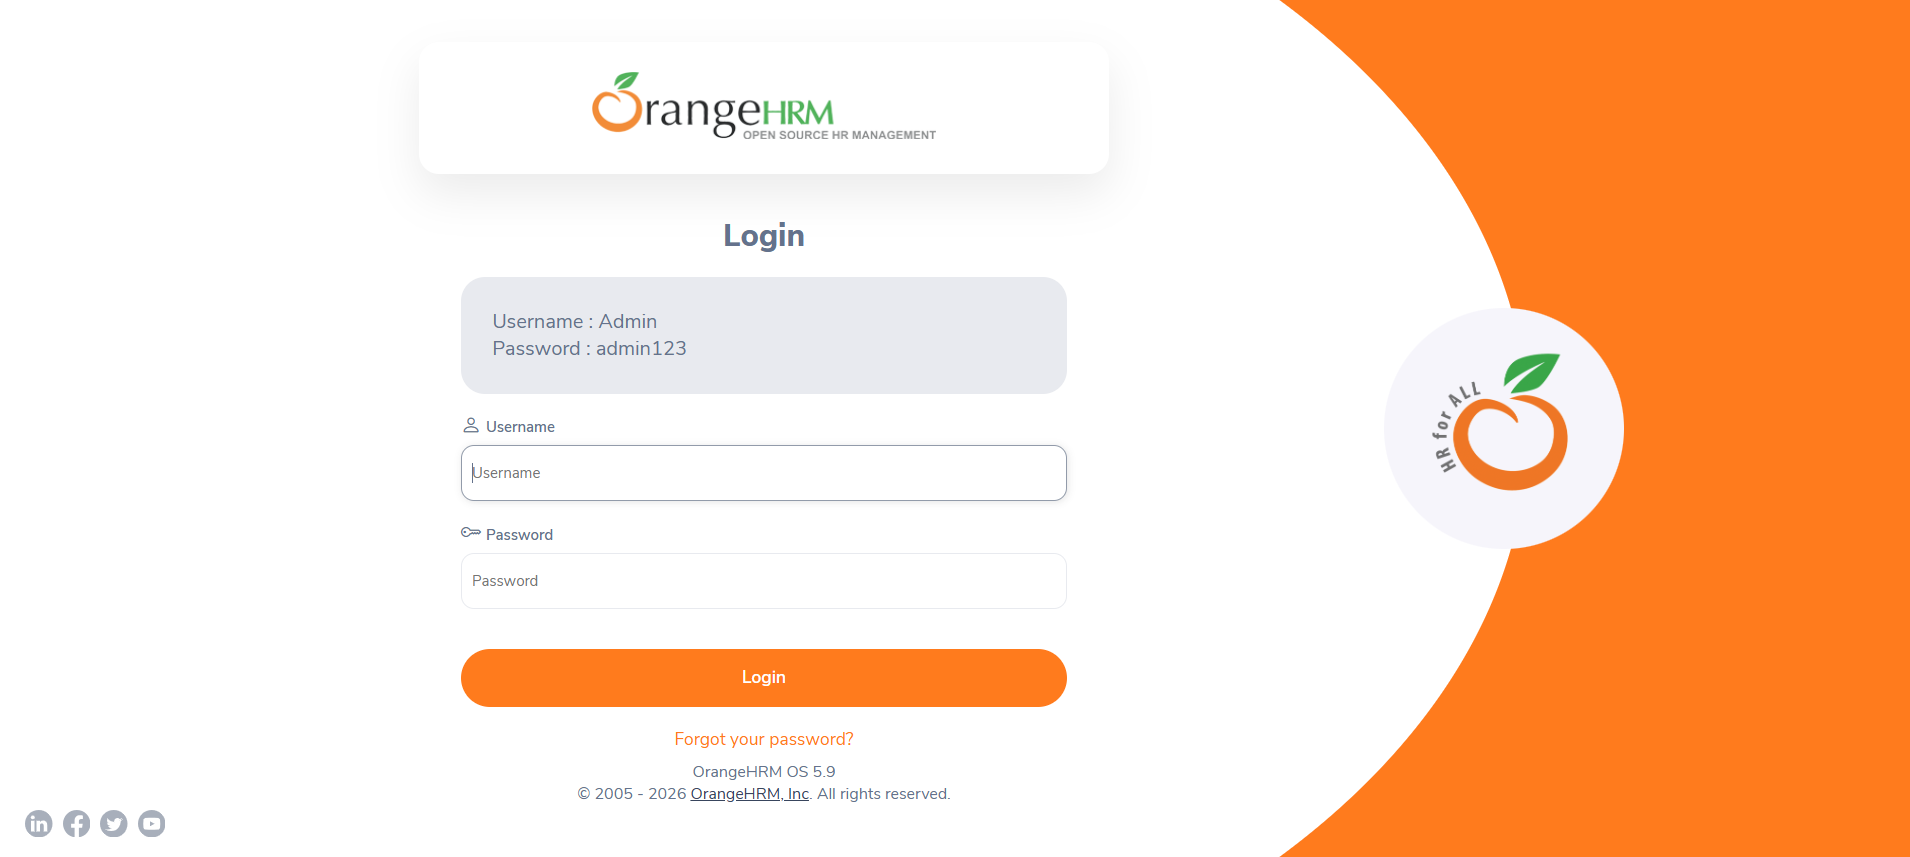
\includegraphics[width=0.85\textwidth]{../screenshots/TS-01_login_page.png}
  \caption{TS-01 - Login page}
\end{figure}

\begin{figure}[H]
  \centering
  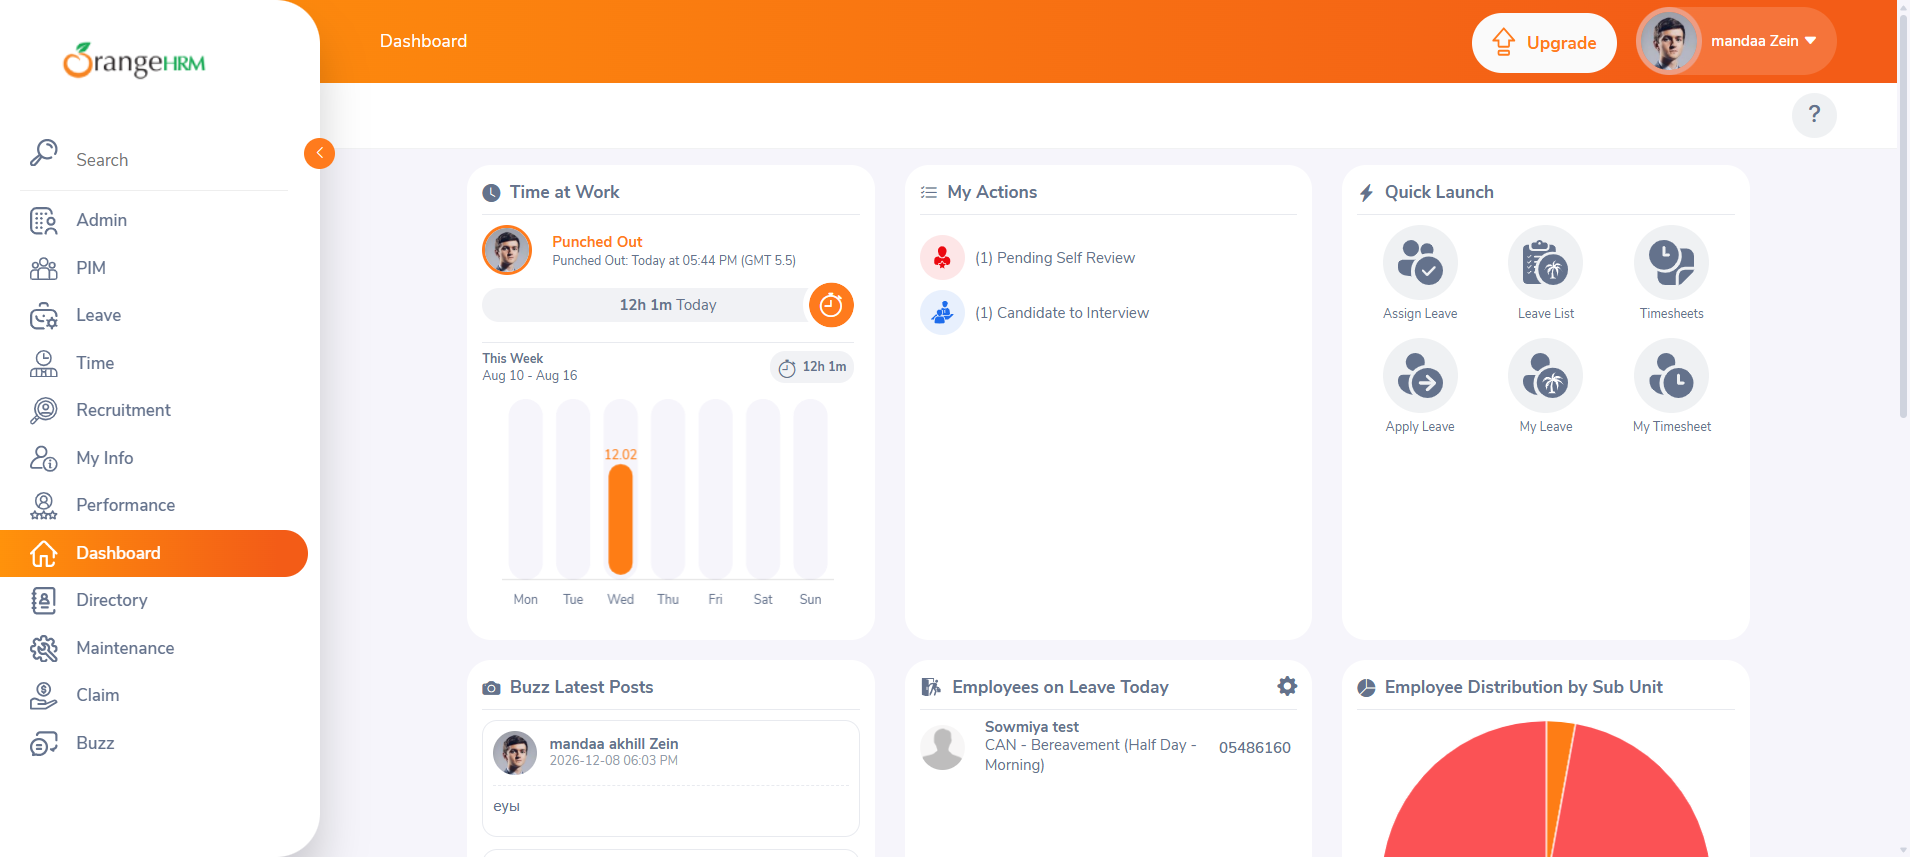
\includegraphics[width=0.85\textwidth]{../screenshots/TS-01_dashboard_after_login.png}
  \caption{TS-01 - Dashboard after successful login}
\end{figure}

\subsection{TS-02 - Invalid Login}
\textbf{Steps:} Enter invalid username/password $\rightarrow$ Click Login\\
\textbf{Expected:} ``Invalid credentials'' error; remain on login page

\begin{figure}[H]
  \centering
  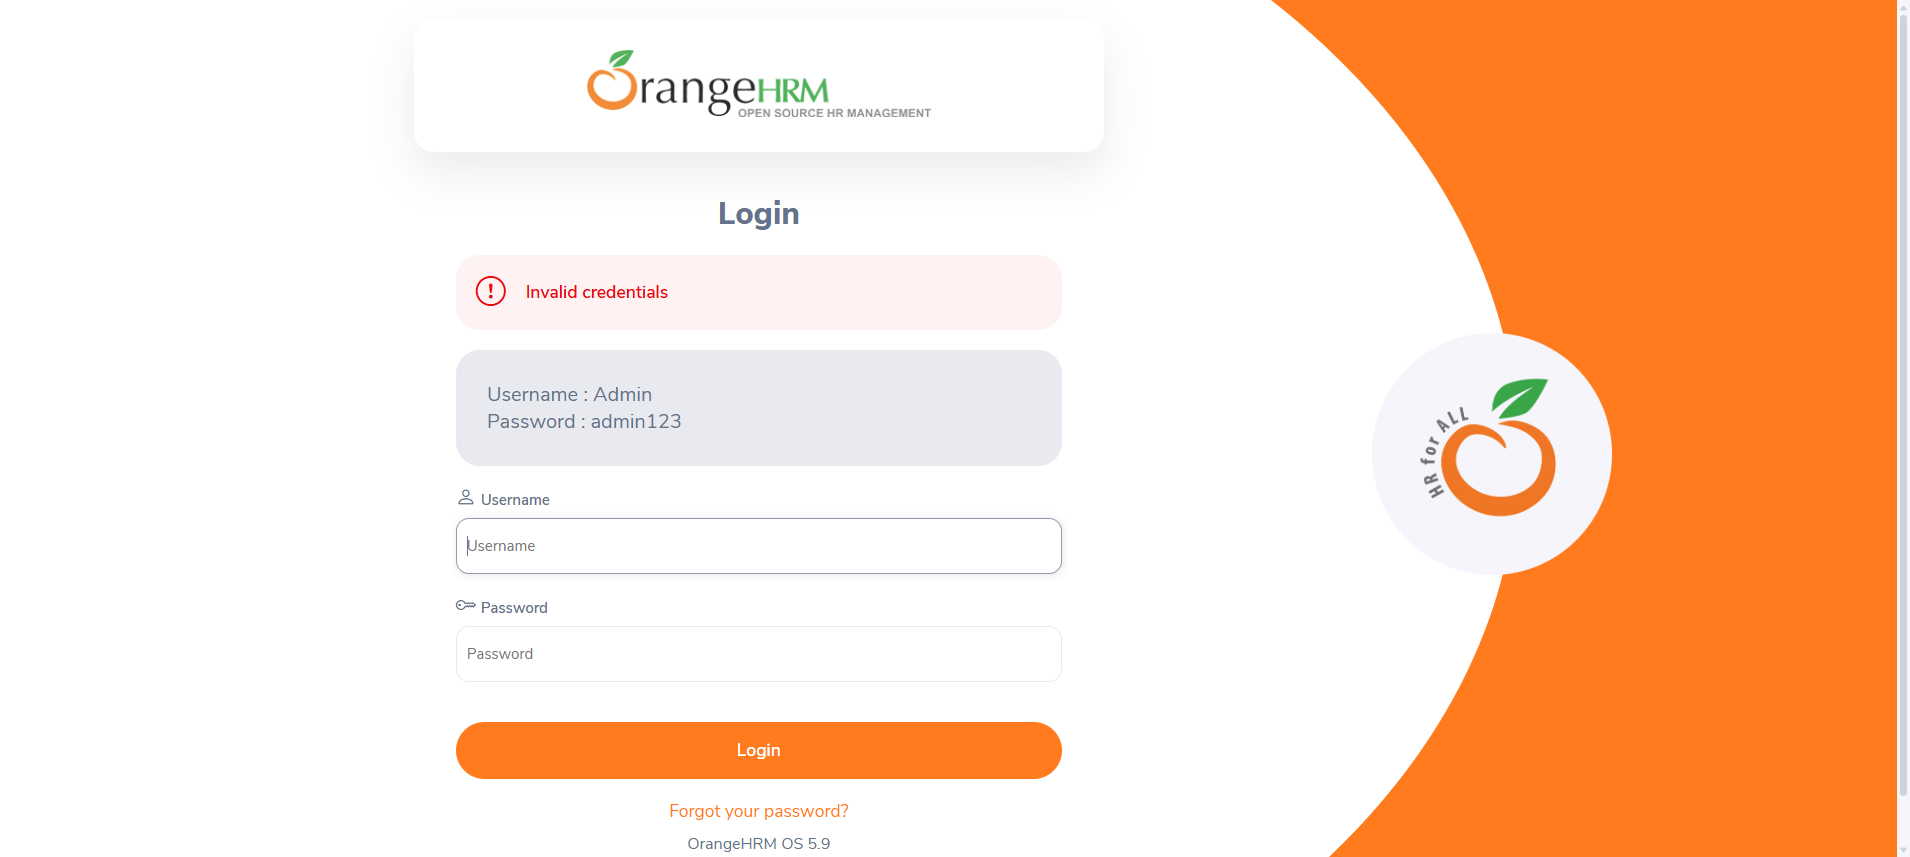
\includegraphics[width=0.85\textwidth]{../screenshots/TS-02_invalid_login_error.png}
  \caption{TS-02 - Invalid login error message}
\end{figure}

\subsection{TS-05 - Dashboard Loads}
\begin{figure}[H]
  \centering
  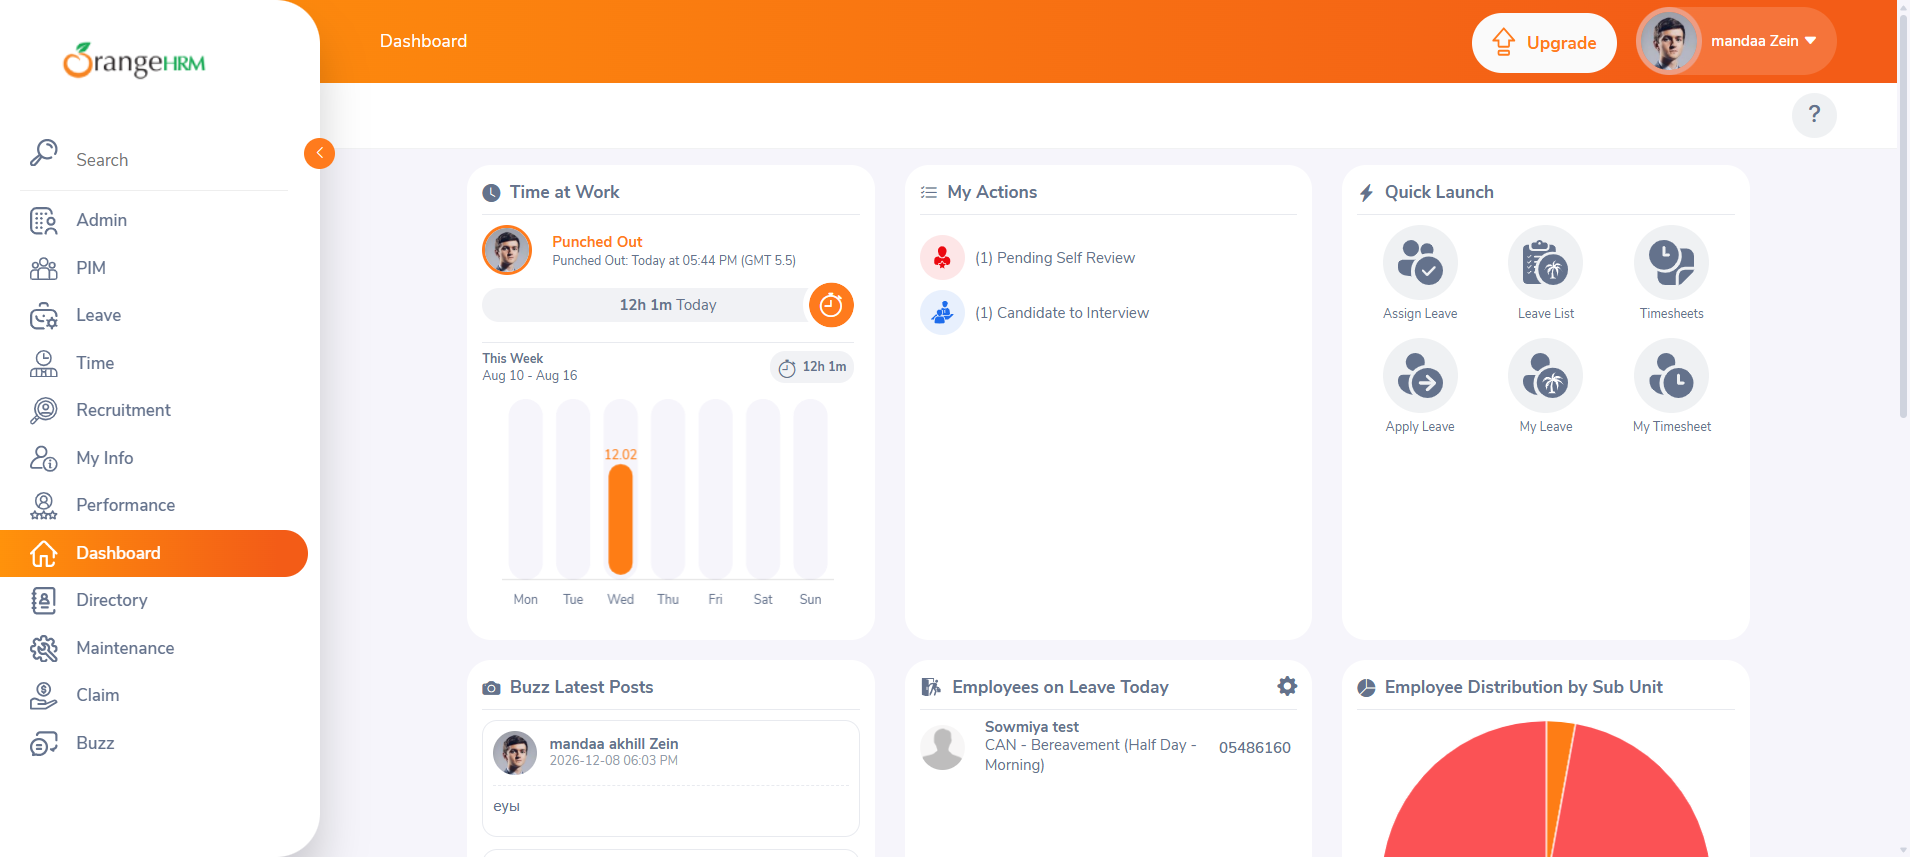
\includegraphics[width=0.85\textwidth]{../screenshots/TS-05_dashboard_widgets.png}
  \caption{TS-05 - Dashboard widgets visible after login}
\end{figure}

\subsection{TS-06 - Navigate to PIM}
\textbf{Expected:} PIM page opens; URL contains \texttt{pim}

\begin{figure}[H]
  \centering
  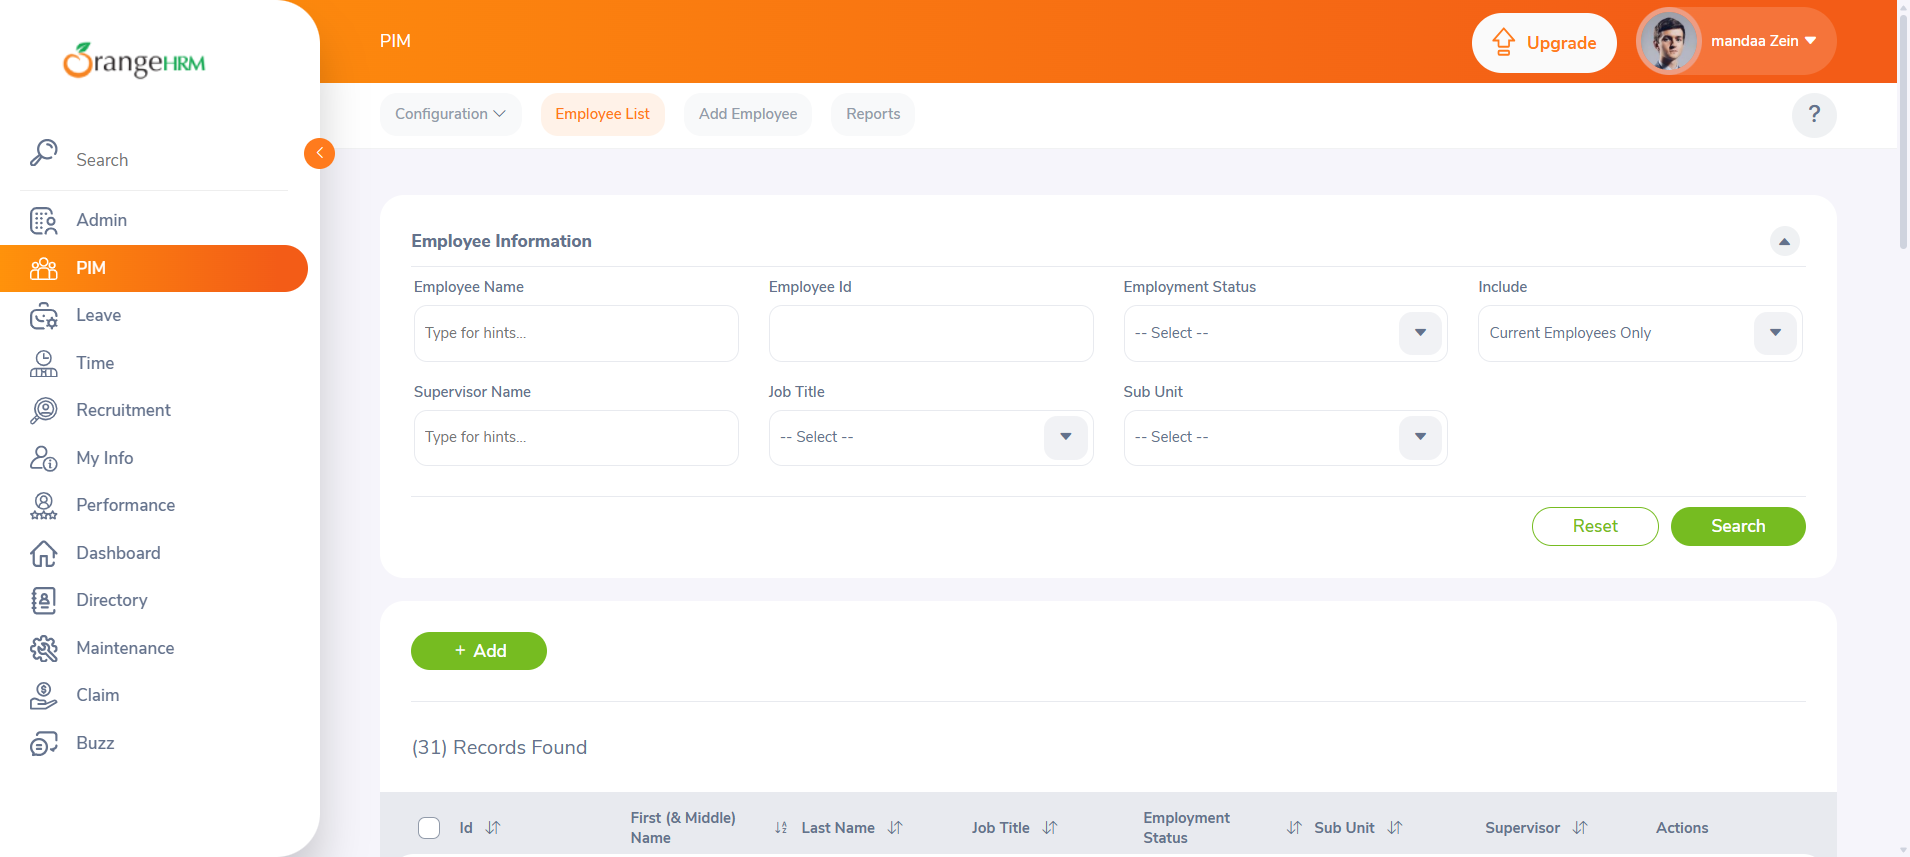
\includegraphics[width=0.85\textwidth]{../screenshots/TS-06_pim_module.png}
  \caption{TS-06 - PIM module}
\end{figure}

\subsection{TS-09 - Admin System Users}
\textbf{Expected:} Admin module opens; ``System Users'' section visible

\begin{figure}[H]
  \centering
  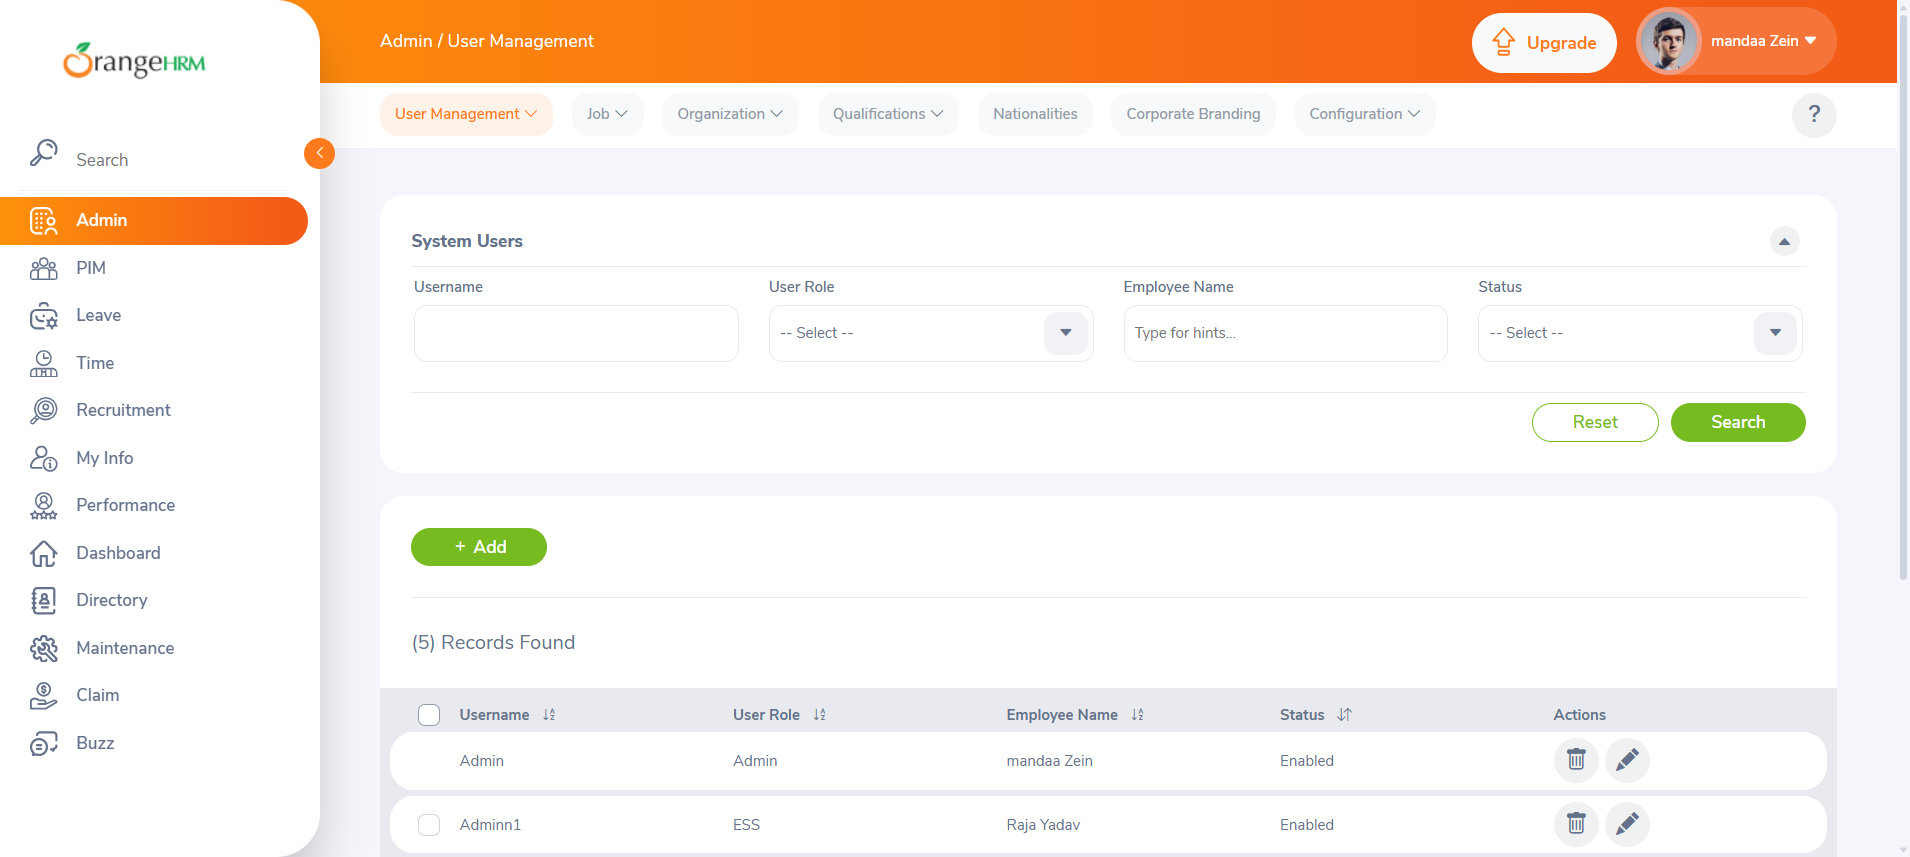
\includegraphics[width=0.85\textwidth]{../screenshots/TS-09_admin_system_users.png}
  \caption{TS-09 - Admin System Users section}
\end{figure}

% ============================================================
\section{Automation Decision}
% ============================================================

\subsection{Selected for Automation (5 scenarios)}
\begin{table}[H]
\centering
\begin{tabular}{@{}clp{6.5cm}@{}}
\toprule
\textbf{ID} & \textbf{Scenario} & \textbf{Why automate} \\
\midrule
TS-01 & Valid login & Critical path; stable locators; strong regression ROI \\
TS-02 & Invalid login & Negative auth; deterministic error message \\
TS-04 & Logout & Security-related; clear URL/state check \\
TS-07 & PIM search & Navigation + form + table coverage \\
TS-09 & Admin users & Second major module; menu + search validation \\
\bottomrule
\end{tabular}
\end{table}

\subsection{Not Automated (examples)}
\begin{itemize}[noitemsep]
  \item \textbf{TS-03} Empty credentials - overlaps TS-02; brittle UI validation
  \item \textbf{TS-08} Add Employee - creates data on shared demo; cleanup unreliable
  \item \textbf{TS-11} Leave flows - date pickers increase complexity
  \item \textbf{TS-12/16} Visual/UX checks - low automation value
  \item \textbf{TS-13} Forgot password - external/environment dependent
\end{itemize}

\noindent\textbf{Decision rule:} Prefer high priority, stable UI, low data side-effects, reusable smoke coverage.

% ============================================================
\section{Framework Design}
% ============================================================

\subsection{Technology Choices}
\begin{itemize}[noitemsep]
  \item \textbf{Java 17} - industry-standard for Selenium
  \item \textbf{Maven} - dependency and build management
  \item \textbf{Selenium 4} - browser automation
  \item \textbf{TestNG} - test lifecycle, suite XML, assertions
  \item \textbf{Page Object Model} - separates UI from test logic
\end{itemize}

\subsection{Package Structure}
\begin{lstlisting}
src/main/java/com/asqa/orangehrm/
  base/    BasePage (shared page helpers)
  pages/   LoginPage, DashboardPage, PIMPage, AdminPage
  utils/   ConfigReader, WaitUtils, ScreenshotUtils
src/test/java/com/asqa/orangehrm/
  base/    BaseTest (browser lifecycle)
  tests/   Five automated scenario classes
src/test/resources/
  config.properties, testng.xml
\end{lstlisting}

\begin{table}[H]
\centering
\begin{tabular}{@{}lp{9cm}@{}}
\toprule
\textbf{Package} & \textbf{Responsibility} \\
\midrule
\texttt{base} & Shared driver/page setup \\
\texttt{pages} & Locators and user actions (no TestNG asserts) \\
\texttt{utils} & Config, waits, screenshots \\
\texttt{tests} & Arrange-Act-Assert only \\
\texttt{resources} & Externalised config and suite XML \\
\bottomrule
\end{tabular}
\end{table}

\subsection{Design Principles}
\begin{enumerate}[noitemsep]
  \item One browser session per \texttt{@Test} method
  \item Explicit waits preferred over fixed sleeps
  \item Screenshots captured on failure via \texttt{@AfterMethod}
  \item Credentials stored in \texttt{config.properties}
\end{enumerate}

% ============================================================
\section{Automation Development}
% ============================================================

\begin{table}[H]
\centering
\begin{tabular}{@{}lll@{}}
\toprule
\textbf{Test Class} & \textbf{Manual ID} & \textbf{Description} \\
\midrule
\texttt{LoginValidTest} & TS-01 & Valid Admin login $\rightarrow$ Dashboard \\
\texttt{LoginInvalidTest} & TS-02 & Invalid credentials $\rightarrow$ error \\
\texttt{LogoutTest} & TS-04 & Logout $\rightarrow$ login URL \\
\texttt{PIMSearchEmployeeTest} & TS-07 & Open PIM $\rightarrow$ search \\
\texttt{AdminUserManagementNavigationTest} & TS-09 & Admin $\rightarrow$ System Users \\
\bottomrule
\end{tabular}
\end{table}

\noindent\textbf{Run command:}
\begin{lstlisting}
mvn clean test
\end{lstlisting}

\noindent All five automated tests pass successfully on Microsoft Edge.

% ============================================================
\section{Debugging Challenge}
% ============================================================

\subsection{Intentional Failure}
The login button locator in \texttt{LoginPage.java} was changed from:
\begin{lstlisting}
private final By loginButton = By.cssSelector("button[type='submit']");
\end{lstlisting}
to an incorrect selector:
\begin{lstlisting}
private final By loginButton = By.cssSelector("button#login-btn-missing");
\end{lstlisting}

\subsection{Observed Failure}
\begin{itemize}[noitemsep]
  \item \textbf{Test:} \texttt{LoginValidTest.validLogin\_shouldOpenDashboard}
  \item \textbf{Exception:} \texttt{TimeoutException} waiting for \texttt{button\#login-btn-missing}
  \item \textbf{Stack trace:} \texttt{WaitUtils.clickable} $\rightarrow$ \texttt{BasePage.click} $\rightarrow$ \texttt{LoginPage.clickLogin}
\end{itemize}

\begin{figure}[H]
  \centering
  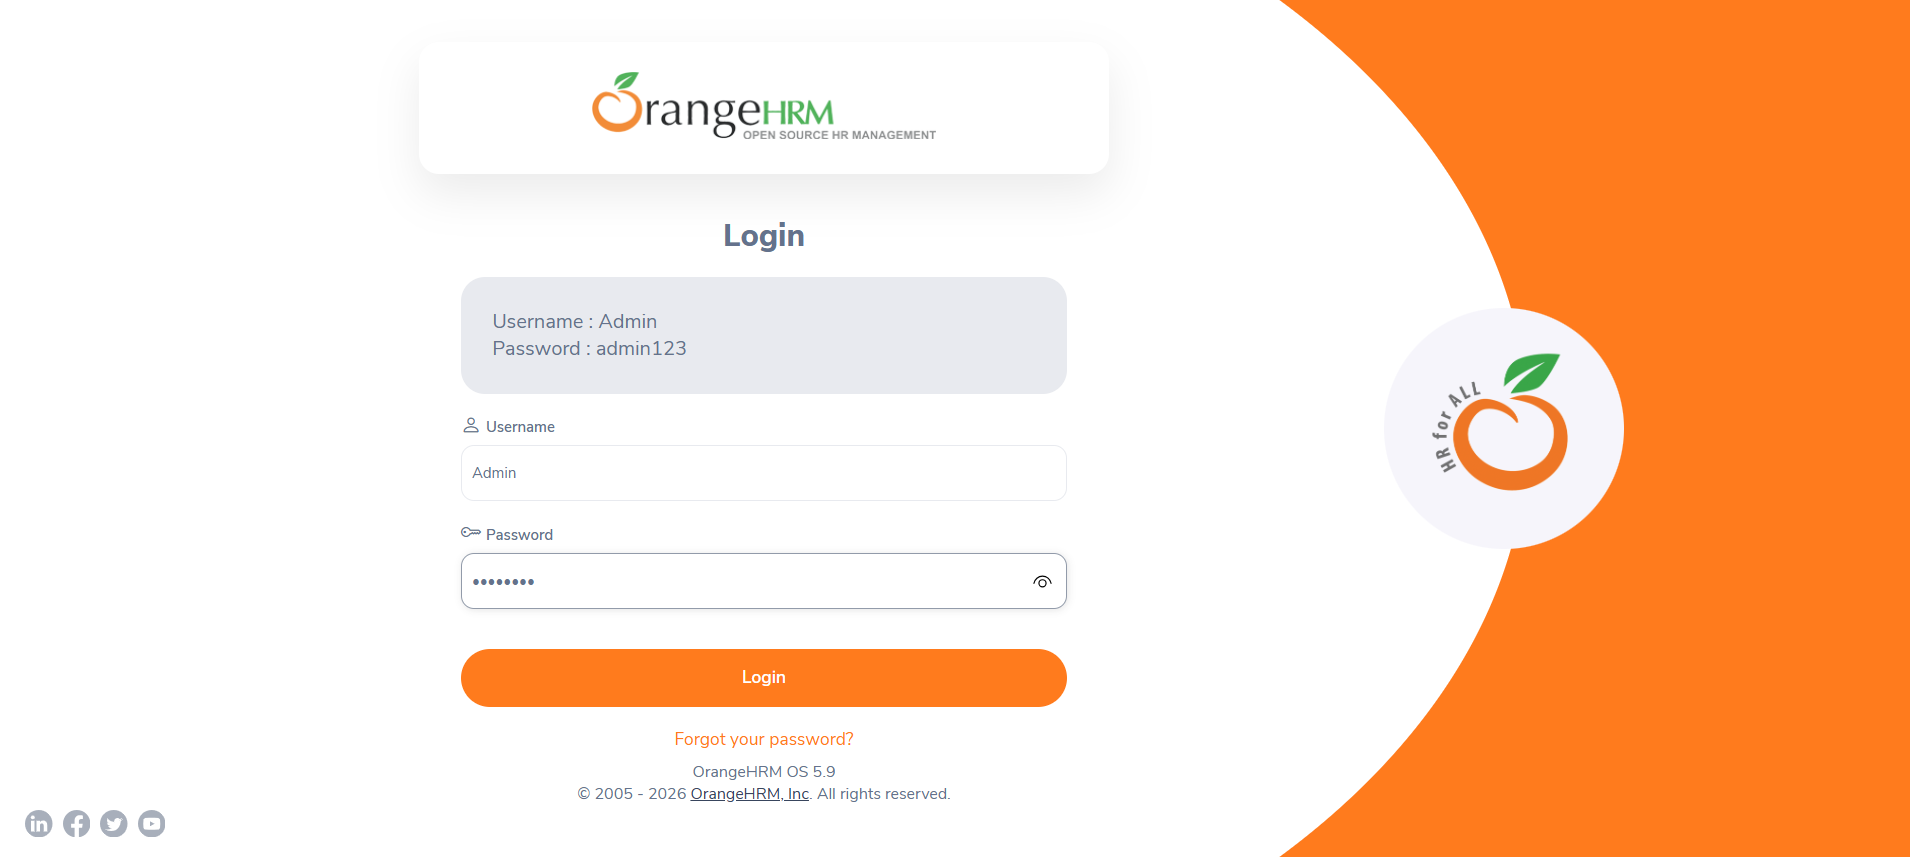
\includegraphics[width=0.85\textwidth]{../debugging/debug_failure_login_button.png}
  \caption{Debugging challenge - failure screenshot (login page visible, wrong locator)}
\end{figure}

\subsection{Debugging Process}
\begin{enumerate}[noitemsep]
  \item Read Surefire stack trace - pointed to login button wait timeout
  \item Opened failure screenshot - page loaded but element not found
  \item Inspected DOM - real button is \texttt{button[type='submit']}
  \item Restored correct locator in \texttt{LoginPage} only (POM benefit)
  \item Re-ran test - \textbf{BUILD SUCCESS}
\end{enumerate}

\subsection{Root Cause and Fix}
\textbf{Root cause:} Invented CSS ID does not exist in OrangeHRM login DOM.\\
\textbf{Fix:} Restored \texttt{button[type='submit']}. Evidence logs in \texttt{docs/debugging/}.

% ============================================================
\section{Reflection Video}
% ============================================================

A five-minute screen recording explaining the implementation and lessons learned is available at:

\begin{center}
\url{https://drive.google.com/file/d/1LVjVxsYdon5JppayyAF42kQZpBJ2Ra5C/view?usp=sharing}
\end{center}

\noindent File name: \texttt{22020782-sqa.mp4}

The recording covers:
\begin{itemize}[noitemsep]
  \item Project structure walkthrough
  \item Running \texttt{mvn clean test}
  \item Page object and test class explanation
  \item Debugging challenge (before/after)
  \item Lessons learned (waits, POM, shared demo risks)
\end{itemize}

% ============================================================
\section{GitHub Repository}
% ============================================================

Incremental commit history maintained at:\\
\url{https://github.com/SeniruR/QA-Automation-ASQA}

\noindent Commits follow logical progression: project setup $\rightarrow$ base utilities $\rightarrow$ page objects $\rightarrow$ tests $\rightarrow$ documentation $\rightarrow$ submission assets.

\vfill
\begin{center}
\small\textit{End of Report - R.P.S.R. Ranasinghe (22020782)}
\end{center}

\end{document}
